\documentclass[review,12pt]{elsarticle}
\usepackage[T1]{fontenc}
\usepackage{amsmath,amssymb,amsthm,booktabs,graphicx,placeins}
\usepackage[a4paper,margin=25mm]{geometry}
\usepackage{microtype}
\usepackage{xurl}
\usepackage[hidelinks]{hyperref}
\hypersetup{pdfauthor={Junyi Zhang},pdftitle={Retention-constrained class expansion with reference-anchored candidate tables}}
\pdfstringdefDisableCommands{\def\corref#1{}\def\cnotenum#1{}}
\newtheorem{proposition}{Proposition}
\newtheorem{corollary}{Corollary}
\newcommand{\RefBase}{86.03}
\newcommand{\RefBaseSD}{1.40}
\newcommand{\RefNovel}{66.90}
\newcommand{\RefNovelSD}{4.23}
\newcommand{\RefAll}{76.46}
\newcommand{\RefAllSD}{1.43}
\newcommand{\RefHarmonic}{75.19}
\newcommand{\RefHarmonicSD}{2.14}
\newcommand{\DynamicBase}{85.36}
\newcommand{\DynamicBaseSD}{0.66}
\newcommand{\DynamicNovel}{70.83}
\newcommand{\DynamicNovelSD}{4.33}
\newcommand{\DynamicAll}{78.09}
\newcommand{\DynamicAllSD}{2.02}
\newcommand{\DynamicHarmonic}{77.36}
\newcommand{\DynamicHarmonicSD}{2.48}
\newcommand{\SimpleBase}{82.47}
\newcommand{\SimpleBaseSD}{0.87}
\newcommand{\SimpleNovel}{77.53}
\newcommand{\SimpleNovelSD}{0.47}
\newcommand{\SimpleAll}{80.00}
\newcommand{\SimpleAllSD}{0.56}
\newcommand{\SimpleHarmonic}{79.92}
\newcommand{\SimpleHarmonicSD}{0.55}
\newcommand{\TextBase}{78.32}
\newcommand{\TextBaseSD}{0.25}
\newcommand{\TextNovel}{76.86}
\newcommand{\TextNovelSD}{1.97}
\newcommand{\TextAll}{77.59}
\newcommand{\TextAllSD}{0.86}
\newcommand{\TextHarmonic}{77.57}
\newcommand{\TextHarmonicSD}{0.88}
\newcommand{\RefErrorFlip}{1.84}
\newcommand{\RefErrorFlipSD}{1.54}
\newcommand{\RefChurn}{3.63}
\newcommand{\RefChurnSD}{2.40}
\newcommand{\LatencyFifty}{1.76}
\newcommand{\LatencySixty}{0.75}
\newcommand{\LatencyEighty}{0.78}
\newcommand{\PetRefBase}{97.18}
\newcommand{\PetRefBaseSD}{2.25}
\newcommand{\PetRefNovel}{87.79}
\newcommand{\PetRefNovelSD}{6.18}
\newcommand{\PetRefAll}{92.49}
\newcommand{\PetRefAllSD}{2.83}
\newcommand{\PetRefHarmonic}{92.14}
\newcommand{\PetRefHarmonicSD}{3.23}
\newcommand{\PetDynamicBase}{96.85}
\newcommand{\PetDynamicBaseSD}{1.50}
\newcommand{\PetDynamicNovel}{86.49}
\newcommand{\PetDynamicNovelSD}{7.64}
\newcommand{\PetDynamicAll}{91.67}
\newcommand{\PetDynamicAllSD}{4.56}
\newcommand{\PetDynamicHarmonic}{91.29}
\newcommand{\PetDynamicHarmonicSD}{4.99}
\newcommand{\PetSimpleBase}{94.77}
\newcommand{\PetSimpleBaseSD}{2.91}
\newcommand{\PetSimpleNovel}{93.91}
\newcommand{\PetSimpleNovelSD}{1.55}
\newcommand{\PetSimpleAll}{94.34}
\newcommand{\PetSimpleAllSD}{1.43}
\newcommand{\PetSimpleHarmonic}{94.31}
\newcommand{\PetSimpleHarmonicSD}{1.44}
\newcommand{\PetTextBase}{92.87}
\newcommand{\PetTextBaseSD}{3.37}
\newcommand{\PetTextNovel}{94.05}
\newcommand{\PetTextNovelSD}{1.35}
\newcommand{\PetTextAll}{93.46}
\newcommand{\PetTextAllSD}{1.59}
\newcommand{\PetTextHarmonic}{93.43}
\newcommand{\PetTextHarmonicSD}{1.63}

\newcommand{\CFMatchedBase}{83.48}
\newcommand{\CFMatchedNovel}{75.79}
\newcommand{\CFTunedNovel}{61.36}
\newcommand{\CFDenseNovel}{74.43}
\newcommand{\CFMatchedGain}{14.43}
\newcommand{\CFDenseGain}{1.37}
\newcommand{\PetStrictBase}{96.84}
\newcommand{\PetStrictNovel}{90.99}
\newcommand{\PetStrictDenseNovel}{84.00}
\newcommand{\PetStrictGain}{7.00}
\newcommand{\CFMatchedGainSD}{6.59}
\newcommand{\CFDenseGainSD}{3.37}
\newcommand{\PetStrictGainSD}{5.57}
\newcommand{\CFTunedAverageGain}{2.18}
\newcommand{\CFTunedAverageGainSD}{0.24}
\newcommand{\CFTunedFinalGain}{1.75}
\newcommand{\CFTunedFinalGainSD}{0.23}
\newcommand{\CFDenseAverageGain}{0.46}
\newcommand{\CFDenseAverageGainSD}{0.44}
\newcommand{\CFDenseFinalGain}{0.02}
\newcommand{\CFDenseFinalGainSD}{0.56}
\newcommand{\CFRemovedAverageGain}{10.62}
\newcommand{\CFRemovedAverageGainSD}{15.22}
\newcommand{\CFRemovedFinalGain}{11.28}
\newcommand{\CFRemovedFinalGainSD}{16.33}
\newcommand{\PetTunedAverageGain}{-0.11}
\newcommand{\PetTunedAverageGainSD}{0.56}
\newcommand{\PetTunedFinalGain}{-0.80}
\newcommand{\PetTunedFinalGainSD}{0.85}
\newcommand{\PetDenseAverageGain}{-0.26}
\newcommand{\PetDenseAverageGainSD}{1.82}
\newcommand{\PetDenseFinalGain}{-0.72}
\newcommand{\PetDenseFinalGainSD}{2.65}
\newcommand{\PetRemovedAverageGain}{16.92}
\newcommand{\PetRemovedAverageGainSD}{28.33}
\newcommand{\PetRemovedFinalGain}{14.92}
\newcommand{\PetRemovedFinalGainSD}{26.40}

\usepackage{xr}\externaldocument[main-]{main}
\begin{document}
\title{Supplementary material: Retention-constrained class expansion with reference-anchored candidate tables}
\author{Junyi Zhang}
\date{}
\maketitle
\appendix
\renewcommand{\thetable}{S\arabic{table}}
\renewcommand{\thefigure}{S\arabic{figure}}

\section{Auxiliary readout and mechanism analyses}
\label{app:auxiliary}
For the auxiliary readout and support-budget comparisons, the gate grid is $a,u\in\{0,0.25,0.5,1,2\}$ and $d\in\{-2,-1.5,\ldots,2\}$. Offset-calibrated controls use their separately stated grids. The main retention/value evaluation uses the common expanded grid in Section~\ref{main-sec:calibration}. All experiments share the same frozen representations, true class partitions and disjoint support pools.

\subsection{Readouts and evaluation measures}
All compared readouts use the same CLIP image embeddings, text anchors, class partitions, and novel support images. The text baseline uses cosine similarity to class names. The visual prototype baseline uses means of base fitting examples and means of novel support examples. Text--prototype fusion adds the two cosine branches with a mixing coefficient selected on the same pseudo-novel calibration episode; its grid is $\{0,0.25,0.5,1,2,4\}$, including pure text.

Tip-Adapter uses a balanced $k$-image cache per candidate and scores $100q_T+\alpha q_{\mathrm{cache}}$, with affinity $\exp[\beta(v^\top f(x_i)-1)]$. The same base-only episode selects $\alpha\in\{0,0.5,1,2,4\}$ and $\beta\in\{1,2,5,10\}$. Cache images come from the reserved pool for both groups; base-trained readouts use the full base fitting set.

We also compare raw evidence fusion and candidate-normalized fusion. Raw fusion uses unstandardized text, learned, and prototype scores with the same coefficient grid as the proposed table. Candidate-normalized fusion standardizes text over all active classes, learned scores over the base classes, and prototypes over active novel classes. It shares the base classifier and calibration protocol with reference-anchored fusion. This comparison changes the normalization population while holding the principal evidence sources fixed.

We report macro base accuracy $A_B$, macro novel accuracy $A_N$, all-class macro accuracy, and the harmonic mean in Eq.~\eqref{main-eq:harmonic}. Both datasets use equal numbers of base and novel classes, so all-class macro accuracy is $(A_B+A_N)/2$. On the balanced CIFAR test set this also equals sample accuracy; on Pets the macro measure gives each breed equal weight. Stability measures include maximum absolute change in an existing score, change of the maximizing class restricted to base classes, and prediction changes over the expanded vocabulary. Error flips are reported as fractions of all base test images, not conditional fractions of previously correct images.

\subsection{Recognition after five-shot class expansion}
\begin{table}[t]
\centering
\caption{Five-shot expansion from 40 base classes to 80 classes. All values are accuracy percentages, reported as mean $\pm$ sample standard deviation over three distinct class partitions. All readouts share frozen CLIP features; coefficients are selected using base-only calibration. Base and novel performance jointly specify each operating point.}
\label{tab:expansion}
\resizebox{\linewidth}{!}{\begin{tabular}{lrrrr}
\toprule
Readout & Base & Novel & All & Harmonic \\
\midrule
CLIP text & 78.32 $\pm$ 0.25 & 76.86 $\pm$ 1.97 & 77.59 $\pm$ 0.86 & 77.57 $\pm$ 0.88 \\
Visual prototypes & 77.53 $\pm$ 2.03 & 60.92 $\pm$ 3.94 & 69.23 $\pm$ 2.09 & 68.17 $\pm$ 2.49 \\
Text + prototypes & 82.47 $\pm$ 0.87 & 77.53 $\pm$ 0.47 & 80.00 $\pm$ 0.56 & 79.92 $\pm$ 0.55 \\
Tip-Adapter (tuned) & 78.38 $\pm$ 0.24 & 77.42 $\pm$ 1.72 & 77.90 $\pm$ 0.83 & 77.89 $\pm$ 0.83 \\
Raw evidence fusion & 78.32 $\pm$ 0.25 & 76.86 $\pm$ 1.97 & 77.59 $\pm$ 0.86 & 77.57 $\pm$ 0.88 \\
Candidate-normalized table & 85.36 $\pm$ 0.66 & 70.83 $\pm$ 4.33 & 78.09 $\pm$ 2.02 & 77.36 $\pm$ 2.48 \\
Reference-anchored table & 86.03 $\pm$ 1.40 & 66.90 $\pm$ 4.23 & 76.46 $\pm$ 1.43 & 75.19 $\pm$ 2.14 \\
\bottomrule
\end{tabular}}
\end{table}

Reference-anchored fusion reaches $\RefBase\pm\RefBaseSD$ base accuracy and $\RefNovel\pm\RefNovelSD$ novel accuracy (Table~\ref{tab:expansion}). Its base accuracy is 7.71 percentage points above text-only classification and 3.56 points above text--prototype fusion, providing a retention-oriented operating point for class expansion.

Text--prototype fusion uses visual evidence for every class and reaches $\SimpleAll\pm\SimpleAllSD$ all-class accuracy and $\SimpleNovel\pm\SimpleNovelSD$ novel accuracy. Candidate-normalized fusion reaches $\DynamicBase\pm\DynamicBaseSD$ base and $\DynamicNovel\pm\DynamicNovelSD$ novel accuracy. These points characterize the recognition trade-off accompanying the reference-anchored score system.

Raw fusion selects the text-only point in all five-shot CIFAR partitions. Both normalization rules activate learned evidence in their selected solutions, demonstrating the role of scale alignment when combining classifier logits with cosine similarities.

\subsection{Fine-grained expansion on Oxford-IIIT Pets}
\begin{table}[t]
\centering
\caption{Five-shot Oxford-IIIT Pets expansion from 15 to 30 breeds under long-tailed base supervision. Values are macro accuracy percentages, mean $\pm$ sample standard deviation across three distinct breed partitions. Grids and the base-only calibration rule are transferred from the CIFAR experiment without dataset-specific search expansion.}
\label{tab:pets}
\resizebox{\linewidth}{!}{\begin{tabular}{lrrrr}
\toprule
Readout & Base & Novel & All & Harmonic \\
\midrule
CLIP text & 92.87 $\pm$ 3.37 & 94.05 $\pm$ 1.35 & 93.46 $\pm$ 1.59 & 93.43 $\pm$ 1.63 \\
Visual prototypes & 92.08 $\pm$ 2.61 & 68.30 $\pm$ 4.62 & 80.19 $\pm$ 2.33 & 78.35 $\pm$ 2.97 \\
Text + prototypes & 94.77 $\pm$ 2.91 & 93.91 $\pm$ 1.55 & 94.34 $\pm$ 1.43 & 94.31 $\pm$ 1.44 \\
Tip-Adapter (tuned) & 93.56 $\pm$ 2.45 & 94.07 $\pm$ 1.18 & 93.81 $\pm$ 1.27 & 93.80 $\pm$ 1.28 \\
Raw evidence fusion & 90.13 $\pm$ 8.01 & 91.18 $\pm$ 4.27 & 90.66 $\pm$ 6.13 & 90.63 $\pm$ 6.18 \\
Candidate-normalized table & 96.85 $\pm$ 1.50 & 86.49 $\pm$ 7.64 & 91.67 $\pm$ 4.56 & 91.29 $\pm$ 4.99 \\
Reference-anchored table & 97.18 $\pm$ 2.25 & 87.79 $\pm$ 6.18 & 92.49 $\pm$ 2.83 & 92.14 $\pm$ 3.23 \\
\bottomrule
\end{tabular}}
\end{table}

On fine-grained Pets expansion, reference anchoring reaches $\PetRefBase\pm\PetRefBaseSD$ base and $\PetRefNovel\pm\PetRefNovelSD$ novel accuracy (Table~\ref{tab:pets}). Base accuracy is 2.41 points above text--prototype fusion. Mean base/novel accuracy also increases from $\PetDynamicBase$\%/$\PetDynamicNovel$\% with candidate normalization to $\PetRefBase$\%/$\PetRefNovel$\% with reference anchoring.

Text--prototype fusion reaches $\PetSimpleAll\pm\PetSimpleAllSD$ all-class macro accuracy; the reference-anchored table reaches $\PetRefAll\pm\PetRefAllSD$ with greater retention of base-breed discrimination. Both datasets use the same search grids and base-only calibration rule.

\subsection{Calibration controls and analytic incremental readouts}
\begin{table}[t]
\centering
\caption{Additional five-shot controls with the same frozen encoder, support images, and base-only calibration. Values are mean $\pm$ sample standard deviation across three partitions. The random-projection readout is a controlled frozen RanPAC-style adaptation described in the text.}
\label{tab:controls}
\small
\begin{minipage}{.49\textwidth}\centering CIFAR-100\\[3pt]\resizebox{\linewidth}{!}{\begin{tabular}{lrrr}
\toprule
Readout & Base & Novel & All \\
\midrule
Text + group offset & 78.93 $\pm$ 2.75 & 75.56 $\pm$ 4.40 & 77.24 $\pm$ 0.89 \\
Anchored text + prototypes & 82.40 $\pm$ 2.02 & 76.19 $\pm$ 3.18 & 79.30 $\pm$ 0.59 \\
Frozen RP-ridge (2000) & 70.18 $\pm$ 0.69 & 52.52 $\pm$ 4.27 & 61.35 $\pm$ 1.83 \\
\bottomrule
\end{tabular}}\end{minipage}\hfill
\begin{minipage}{.49\textwidth}\centering Oxford-IIIT Pets\\[3pt]\resizebox{\linewidth}{!}{\begin{tabular}{lrrr}
\toprule
Readout & Base & Novel & All \\
\midrule
Text + group offset & 95.29 $\pm$ 3.80 & 89.85 $\pm$ 4.86 & 92.57 $\pm$ 2.31 \\
Anchored text + prototypes & 94.58 $\pm$ 3.22 & 90.38 $\pm$ 5.41 & 92.48 $\pm$ 1.10 \\
Frozen RP-ridge (2000) & 93.49 $\pm$ 3.32 & 73.70 $\pm$ 5.13 & 83.60 $\pm$ 1.13 \\
\bottomrule
\end{tabular}}\end{minipage}
\end{table}

Offset-calibrated controls share the same pseudo-novel episode (Table~\ref{tab:controls}). Text + group offset uses base-referenced text scores and a novel offset. Anchored text + prototypes uses fixed base references for both branches and visual evidence for every class. Harmonic selection searches offsets from $-4$ to $4$ in steps of $0.25$ and prototype weights $\{0,0.25,0.5,1,2,4\}$. Fixed-reference text--prototype fusion also satisfies Proposition~\ref{main-prop:invariance}; the score invariant applies across availability masks.

Anchored text--prototype fusion attains 82.40\% base and 76.19\% novel accuracy on CIFAR, and 94.58\%/90.38\% on Pets. Offset-calibrated text attains 78.92\%/75.56\% and 95.29\%/89.85\%, respectively. Together with the heterogeneous table, these controls separate group calibration, evidence configuration, and the shared fixed-reference property.

The analytic baseline follows the random-projection phase of RanPAC~\cite{mcdonnell2023ranpac}. A fixed Gaussian matrix maps CLIP features to 2000 ReLU coordinates, and $(G+\lambda I)W=Q$ accumulates Gram matrices and class cross-products from base fitting data and novel support. Base validation macro accuracy selects $\lambda\in\{10^{-8},\ldots,10^8\}$; the pseudo episode selects a novel offset. This frozen adaptation uses base validation in place of the original within-task MSE selection. It attains 70.18\%/52.53\% base/novel accuracy on CIFAR and 93.49\%/73.70\% on Pets. Novel statistics refit the analytic readout; candidate-table expansion appends rows to its fixed readout.

\begin{table}[t]
\centering
\caption{Validation retention-targeted calibration at five shots. The pseudo-base target is 95\% of the closed reference-table pseudo-base accuracy. Among feasible grid points, selection maximizes pseudo-novel accuracy; infeasible partitions use the point with highest pseudo-base accuracy, then pseudo-novel accuracy. Feasible counts refer to validation partitions. Test values are percentages, mean $\pm$ sample standard deviation; test retention is not constrained.}
\label{tab:retention}
\resizebox{\linewidth}{!}{\begin{tabular}{llrrrr}
\toprule
Data & Readout & Base & Novel & All & Feasible \\
\midrule
CIFAR & Text + group offset & 81.47 $\pm$ 1.13 & 71.49 $\pm$ 5.03 & 76.48 $\pm$ 1.99 & 1/3 \\
CIFAR & Anchored text + prototypes & 82.84 $\pm$ 1.50 & 77.11 $\pm$ 4.46 & 79.98 $\pm$ 1.61 & 3/3 \\
CIFAR & Candidate-normalized table & 84.69 $\pm$ 1.92 & 72.45 $\pm$ 4.14 & 78.57 $\pm$ 1.54 & 3/3 \\
CIFAR & Reference-anchored table & 84.56 $\pm$ 1.31 & 73.88 $\pm$ 5.01 & 79.22 $\pm$ 2.21 & 3/3 \\
Pets & Text + group offset & 95.29 $\pm$ 3.80 & 89.85 $\pm$ 4.86 & 92.57 $\pm$ 2.31 & 3/3 \\
Pets & Anchored text + prototypes & 94.03 $\pm$ 3.37 & 90.96 $\pm$ 5.91 & 92.50 $\pm$ 1.27 & 3/3 \\
Pets & Candidate-normalized table & 97.25 $\pm$ 1.78 & 85.26 $\pm$ 7.25 & 91.26 $\pm$ 4.40 & 3/3 \\
Pets & Reference-anchored table & 97.18 $\pm$ 2.25 & 87.79 $\pm$ 6.18 & 92.49 $\pm$ 2.83 & 3/3 \\
\bottomrule
\end{tabular}}
\end{table}

Under the common 95\% validation retention target, reference anchoring reaches 84.56\% base and 73.87\% novel test accuracy on CIFAR, compared with 82.84\%/77.11\% for anchored text--prototype fusion (Table~\ref{tab:retention}). Both are feasible on all three validation partitions. On Pets, the corresponding test points are 97.18\%/87.79\% and 94.03\%/90.96\%. Text alone reaches the CIFAR validation target in one partition. Targets constrain validation selection; the table reports the resulting test operating points. Complete 95\% and 99\% results accompany the experimental records.

\subsection{Vocabulary growth and score preservation}
\begin{figure}[t]
\centering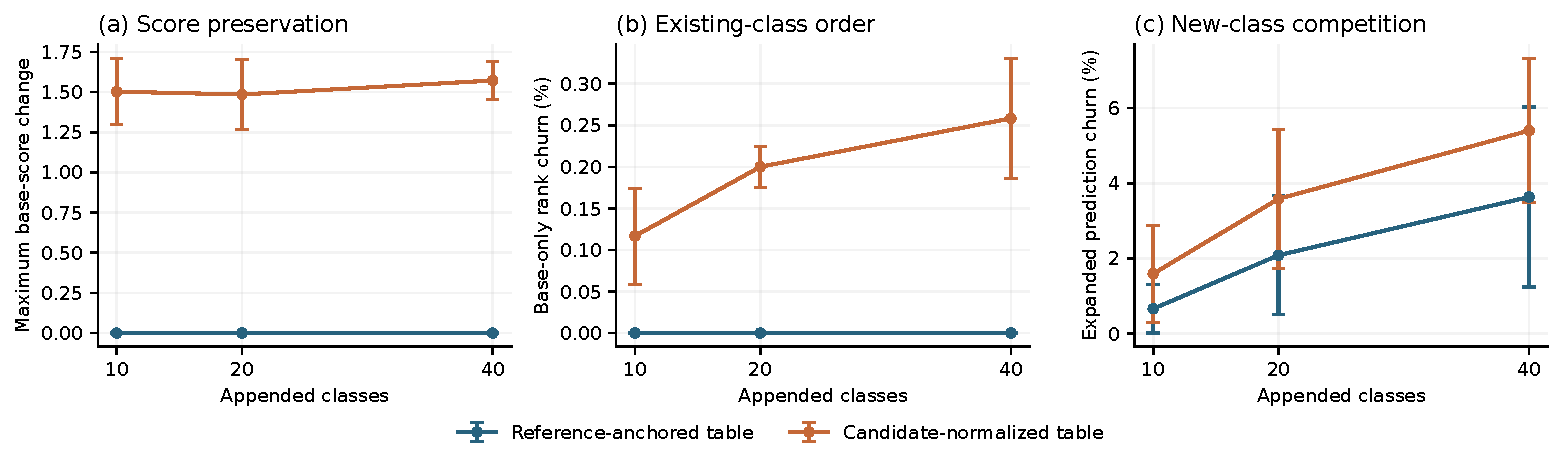
\includegraphics[width=.98\textwidth]{stability.pdf}
\caption{Vocabulary growth with five-shot novel prototypes. Each curve averages three true class partitions; error bars show sample standard deviation. Reference-anchored fusion preserves existing scores and base-only rankings. Expanded predictions can still change when a new candidate wins. Maximum score drift is measured across all test queries and existing base classes.}
\label{fig:stability}
\end{figure}

The vocabulary test appends nested sets of 10, 20, and 40 novel classes to the 40 CIFAR base classes, using sorted novel IDs and fixed five-shot gates. At each stage, we compare existing scores with the original base decision.

Reference anchoring gives zero measured base-score drift and zero base-only ranking churn in all nine CIFAR partition--vocabulary conditions (Fig.~\ref{fig:stability}(a,b)). Candidate normalization changes existing scores by up to approximately 1.29--1.74 normalized units and changes a fraction of base-only predictions. The Pets test appends 3, 7, and 15 breeds and likewise records zero anchored score drift and ranking churn in all nine conditions.

At 40 appended classes, expanded predictions change on $\RefChurn\pm\RefChurnSD$\% of base images, including $\RefErrorFlip\pm\RefErrorFlipSD$\% correct-to-wrong changes (Fig.~\ref{fig:stability}(c)). Wrong-to-correct changes are zero, as specified by Corollary~\ref{cor:competition}. The preserved base scores isolate these changes as competition from appended rows.

Five-session expansion adds eight CIFAR classes or three Pets breeds per session, with two random arrival orders per partition. Across 30 session records per dataset, comparisons of all previously admitted rows, including novel rows, give maximum floating-point score differences of $2.85\times10^{-5}$ on CIFAR and $3.58\times10^{-6}$ on Pets. Both arrival orders produce identical final predictions in every partition under class-ID tie breaking.

\subsection{Support budget and evidence availability}
\begin{table}[t]
\centering
\caption{Reference-anchored expansion across novel support budgets. Accuracy percentages are aggregated across partitions after averaging support subsets within each partition.}
\label{tab:shots}
\resizebox{\linewidth}{!}{\begin{tabular}{lrrrr}
\toprule
Shots & Base & Novel & All & Harmonic \\
\midrule
1 & 84.57 $\pm$ 0.88 & 70.86 $\pm$ 5.41 & 77.72 $\pm$ 2.27 & 77.00 $\pm$ 2.85 \\
2 & 85.65 $\pm$ 1.45 & 70.05 $\pm$ 1.13 & 77.85 $\pm$ 0.67 & 77.04 $\pm$ 0.67 \\
5 & 86.03 $\pm$ 1.40 & 66.90 $\pm$ 4.23 & 76.46 $\pm$ 1.43 & 75.19 $\pm$ 2.14 \\
\bottomrule
\end{tabular}}
\end{table}
\begin{figure}[t]
\centering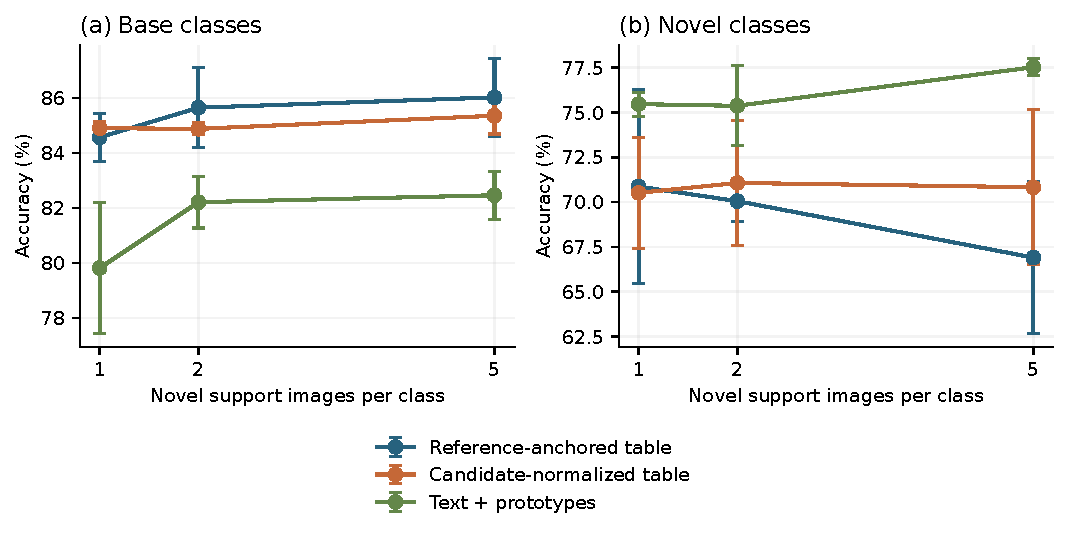
\includegraphics[width=.76\textwidth]{shots.pdf}
\caption{Base and novel accuracy at one, two, and five support images per novel class. The same fixed-reference scoring rule is used at every budget, with coefficients selected on the corresponding base-only pseudo episode. Error bars represent variation between class partitions.}
\label{fig:shots}
\end{figure}

At one, two, and five shots, base accuracy remains between 84.57\% and 86.03\%, while novel accuracy ranges from 66.90\% to 70.86\% (Table~\ref{tab:shots}; Fig.~\ref{fig:shots}). Calibration includes zero branch coefficients, allowing the selected mixture to adapt to the support budget. Each budget defines a separately calibrated operating point: support determines the prototype evidence, and fusion determines its competition with learned base discrimination.

\subsection{Mechanism ablation and operating trade-off}
\begin{table}[t]
\centering
\caption{Evidence removal at the selected five-shot reference-anchored operating point, with all remaining coefficients fixed. Accuracy percentages are mean $\pm$ sample standard deviation over three class partitions.}
\label{tab:ablation}
\resizebox{\linewidth}{!}{\begin{tabular}{lrrrr}
\toprule
Readout & Base & Novel & All & Harmonic \\
\midrule
Reference-anchored table & 86.03 $\pm$ 1.40 & 66.90 $\pm$ 4.23 & 76.46 $\pm$ 1.43 & 75.19 $\pm$ 2.14 \\
Without learned evidence & 58.10 $\pm$ 32.21 & 80.72 $\pm$ 4.47 & 69.41 $\pm$ 13.87 & 62.85 $\pm$ 25.08 \\
Without novel prototypes & 86.42 $\pm$ 1.71 & 47.17 $\pm$ 30.85 & 66.79 $\pm$ 14.62 & 56.15 $\pm$ 30.05 \\
Without offset & 86.14 $\pm$ 1.69 & 65.58 $\pm$ 7.35 & 75.86 $\pm$ 2.83 & 74.25 $\pm$ 4.08 \\
\bottomrule
\end{tabular}}
\end{table}
\begin{figure}[t]
\centering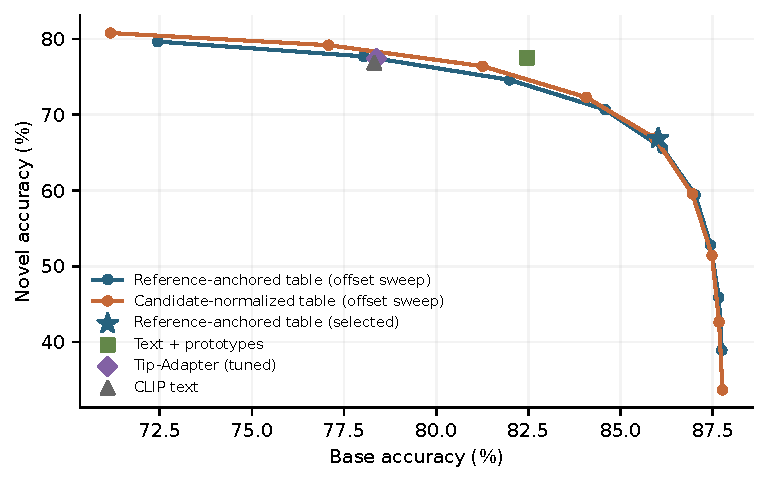
\includegraphics[width=.98\linewidth]{tradeoff.pdf}
\caption{Base--novel operating curves for five-shot expansion. The offset is swept with the other selected coefficients fixed; these test curves are descriptive analyses and are not used to select the reported operating points. Symbols identify base-only calibrated points and matched baselines.}
\label{fig:tradeoff}
\end{figure}

Removing learned evidence, novel prototypes, or the offset changes a different part of the selected decision rule (Table~\ref{tab:ablation}). With the remaining coefficients fixed, these interventions identify how each source contributes to the five-shot operating point. The independently calibrated text and text--prototype readouts provide the corresponding reduced-model comparisons.

Figure~\ref{fig:tradeoff} sweeps $d$ from $-2$ to $2$ in steps of 0.5 with $a$ and $u$ fixed. Increasing $d$ shifts the margin between the best base and novel candidates while preserving within-group rankings (Eq.~\eqref{main-eq:base-novel}). The resulting curve identifies how the offset controls admission of new categories; a validation retention target selects the operating point.

\subsection{Readout efficiency}
Candidate scoring from cached 768-dimensional features takes approximately \LatencyFifty, \LatencySixty, and \LatencyEighty\ ms per batch for 50, 60, and 80 candidates. Measurements use batches of 256 on an NVIDIA RTX 4070 Laptop GPU, five warm-up iterations, and 50 timed iterations with GPU synchronization. They include reference statistics and fusion and exclude image/text encoding. At these vocabulary sizes, launch and reduction overheads dominate the measured latency.


\FloatBarrier
\section{Validation-selected retention policy}
\label{app:validationpolicy}
\begin{table}[t]
\centering
\caption{Final-session test accuracies after the admission threshold is selected using base validation only. Budgets use the same closed-base validation reference for all methods within a partition. Values are percentages, mean $\pm$ sample standard deviation over feasible partitions; counts identify those partitions. Test accuracies are the outcomes of this operational policy and are not matched by test labels.}
\label{tab:validationvalue}
\resizebox{\linewidth}{!}{\begin{tabular}{lllrrr}
\toprule
Data & Budget & Readout & Base & Novel & Feasible \\
\midrule
CIFAR & 90\% & Retained classifier & 78.33 $\pm$ 3.89 & 80.13 $\pm$ 2.25 & 3/3 \\
CIFAR & 90\% & Classifier removed (fixed gates) & 79.07 $\pm$ 3.94 & 70.79 $\pm$ 13.81 & 3/3 \\
CIFAR & 90\% & No classifier (recalibrated) & 78.73 $\pm$ 3.21 & 75.45 $\pm$ 5.43 & 3/3 \\
CIFAR & 90\% & Anchored text + prototypes & 80.18 $\pm$ 0.60 & 79.45 $\pm$ 0.76 & 3/3 \\
CIFAR & 95\% & Retained classifier & 82.99 $\pm$ 2.29 & 75.71 $\pm$ 3.14 & 3/3 \\
CIFAR & 95\% & Classifier removed (fixed gates) & 81.95 $\pm$ 0.04 & 71.54 $\pm$ 3.87 & 2/3 \\
CIFAR & 95\% & No classifier (recalibrated) & 81.85 $\pm$ 0.18 & 71.70 $\pm$ 4.10 & 2/3 \\
CIFAR & 95\% & Anchored text + prototypes & 81.95 $\pm$ 0.64 & 77.48 $\pm$ 1.52 & 2/3 \\
CIFAR & 99\% & Retained classifier & 86.48 $\pm$ 1.65 & 62.83 $\pm$ 10.11 & 3/3 \\
CIFAR & 99\% & Classifier removed (fixed gates) & -- & -- & 0/3 \\
CIFAR & 99\% & No classifier (recalibrated) & -- & -- & 0/3 \\
CIFAR & 99\% & Anchored text + prototypes & 86.85 & 53.85 & 1/3 \\
Pets & 90\% & Retained classifier & 84.87 $\pm$ 4.59 & 96.53 $\pm$ 0.78 & 3/3 \\
Pets & 90\% & Classifier removed (fixed gates) & 84.11 $\pm$ 2.76 & 96.44 $\pm$ 0.64 & 3/3 \\
Pets & 90\% & No classifier (recalibrated) & 82.00 $\pm$ 0.20 & 96.38 $\pm$ 0.52 & 3/3 \\
Pets & 90\% & Anchored text + prototypes & 85.69 $\pm$ 4.62 & 95.87 $\pm$ 1.57 & 3/3 \\
Pets & 95\% & Retained classifier & 90.29 $\pm$ 2.90 & 95.68 $\pm$ 0.83 & 3/3 \\
Pets & 95\% & Classifier removed (fixed gates) & 90.11 $\pm$ 1.17 & 95.71 $\pm$ 0.11 & 2/3 \\
Pets & 95\% & No classifier (recalibrated) & 89.88 $\pm$ 0.85 & 95.71 $\pm$ 0.11 & 2/3 \\
Pets & 95\% & Anchored text + prototypes & 89.37 $\pm$ 4.15 & 95.63 $\pm$ 1.55 & 3/3 \\
Pets & 99\% & Retained classifier & 96.43 $\pm$ 2.15 & 88.67 $\pm$ 7.89 & 3/3 \\
Pets & 99\% & Classifier removed (fixed gates) & -- & -- & 0/3 \\
Pets & 99\% & No classifier (recalibrated) & -- & -- & 0/3 \\
Pets & 99\% & Anchored text + prototypes & 97.70 $\pm$ 1.11 & 84.19 $\pm$ 12.46 & 2/3 \\
\bottomrule
\end{tabular}}
\end{table}
Table~\ref{tab:validationvalue} applies the common validation target after five arrivals. Raw records include all five target fractions and every arrival session. Infeasible targets are reported without substituting a zero novel accuracy. Comparisons with different feasible counts refer to different partition sets.
\FloatBarrier
\section{Reproduction details}
\label{app:reproduction}
The expansion experiment is implemented in \nolinkurl{src/experiments/fcs_expansion.py}. It can be run from any working directory. The manifest records the code hash, frozen-cache hash, image-pool hashes, class assignments, pseudo-class assignments, support indices, regularization choices, and selection grids. The frozen support features are computed with the same deterministic interpolation used for the frozen training cache. The cached image embeddings are checked numerically before scoring.

Every novel support image comes from the five-image-per-class reserve created before long-tail sampling. This supplies a consistent support budget even for tail classes whose fitting pool contains fewer than five images. At five shots the three subset seeds select the same images in different orders, so the reported standard deviation is calculated across the three distinct class partitions. One- and two-shot results average the three subsets within each partition before computing the partition-level variation.

The main result JSON contains all compared readouts, including evidence-removal ablations. The vocabulary records contain the maximum score drift and both restricted and expanded prediction churn. The operating-curve records contain every swept offset, with no selection based on test outcomes. The efficiency records specify batch size and measured vocabulary size. The manuscript tables are generated directly from these files, and the summary CSV exposes both means and sample standard deviations.

The semantic prompts are ``a photo of a \{\}.'', ``a bad photo of a \{\}.'', ``a cropped photo of a \{\}.'', ``a close-up photo of a \{\}.'', ``a bright photo of a \{\}.'', ``a good photo of a \{\}.'', ``a photo of the \{\}.'', and a second occurrence of ``a photo of a \{\}.''. The repeated prompt follows the existing cached anchor construction and is retained consistently for all methods.

Frozen CLIP features are the sole image representation in the expansion experiments. Six fitting images are independently re-embedded and checked for cosine agreement above 0.999 with the cached features. Image hashes verify that fitting, validation, and reserved-support pools are disjoint. The fixed base text block is computed separately from novel text columns; sequential prototype products can exhibit the reported floating-point residuals when matrix widths change.

\section{Interpreting group competition}
Let $M_B(x)=\max_{b\in\mathcal B}[\widehat q_T(x,b)+a\widehat q_L(x,b)]$ and $M_N(x)=\max_{n\in\mathcal N}[\widehat q_T(x,n)+u\widehat q_P(x,n)]$. The classifier selects a novel class precisely when $M_N(x)+d>M_B(x)$, subject to the fixed tie-breaking rule. Hence, the offset is a threshold on the margin $M_B-M_N$. Increasing $d$ cannot change the winning base class or the winning novel class when all other quantities are fixed. It changes which group supplies the final winner. This explains the direction of the operating curves without assuming a calibrated probability interpretation for the fused score.

For nested candidate sets and fixed references, adding novel rows can increase $M_N$ but cannot change $M_B$. An existing-class example may therefore cross the admission boundary as the vocabulary grows, while its base scores remain identical. This distinguishes the deployment behavior measured by expanded prediction churn from the normalization behavior measured by base-only ranking churn.

\FloatBarrier
\section{Additional background and score-preservation proof}
\subsection{Long-tailed recognition and calibration}
Long-tailed recognition addresses the bias induced by unequal class frequencies. Margin adjustment allocates different classification margins to frequent and rare classes~\cite{cao2019ldam}; class-balanced weighting uses effective sample counts~\cite{cui2019classbalanced}; and prior-aware objectives modify the relationship between logits and class probabilities~\cite{ren2020bsm,menon2021logitadj}. Representation--classifier decoupling provides a complementary route: a representation is learned first and a balanced classifier is then fitted to that representation~\cite{kang2020decoupling}. These developments motivate our use of a balanced base classifier as one source of evidence.

Foundation models change the representation-learning budget and the role of task-specific adaptation. LIFT studies lightweight adaptation of pre-trained models for long-tail learning~\cite{shi2024lift}. Low-rank updates provide an efficient mechanism for adapting large parameter matrices~\cite{hu2022lora}, including transformer backbones~\cite{dosovitskiy2021vit}. Our candidate interface can accept weights obtained through these routes. The expansion experiments here fix the encoder throughout and isolate the effect of the readout.

Long-tailed calibration studies confidence under class imbalance~\cite{zhong2021mislas}, while robust long-tailed learning addresses its interaction with label noise~\cite{wei2026robust}. We study the reference population used to standardize evidence as candidate classes change. Class-balanced validation and separate base/novel metrics expose how the resulting score system allocates discrimination.

\subsection{Semantic and visual evidence for few-shot recognition}
CLIP constructs classifiers from natural-language supervision and supports classification by changing the text candidates~\cite{radford2021clip}. CoOp learns prompt context for target tasks, while CoCoOp introduces conditional prompting to improve transfer across categories~\cite{zhou2022coop,zhou2022cocoop}. These methods concern the construction or adaptation of semantic evidence. Our table keeps semantic anchors available to every class and combines them with evidence that may exist for only a subset of the vocabulary.

Prototype methods summarize class examples in an embedding space~\cite{snell2017prototypical}. SimpleShot studies feature normalization for nearest-neighbor classification~\cite{wang2019simpleshot}, and Tip-Adapter augments CLIP with a support-feature cache~\cite{zhang2022tipadapter}. Few-shot transfer under distribution shift further motivates separating shared and task-specific knowledge~\cite{zhu2023combat}. Our comparisons use a shared encoder and novel support budget to examine evidence availability and its normalization reference.

\subsection{Proof of the main score-preservation proposition}
\begin{proof}
For an existing candidate $c$, each raw score $q_e(x,c)$ and mask $m_{ec}$ is fixed. The means and variances in Eq.~\eqref{main-eq:reference} are functions of $x$ and $\mathcal R_e$, and neither depends on the appended rows. Therefore each normalized score in Eq.~\eqref{main-eq:anchored} is unchanged. The coefficients and offset of $c$ are fixed, so their sum is unchanged. Subtracting the unchanged scores of any two existing rows gives an unchanged difference. A fixed tie-breaking rule preserves the maximizing existing row.
\end{proof}

The proposition covers both base rows and previously appended novel rows with fixed prototypes. The implementation computes the fixed base text block separately from novel columns to keep its numerical kernel independent of the appended width.

\begin{corollary}
If every existing row has a preserved score, a changed final prediction after expansion must select an appended row. An example whose previous prediction was incorrect cannot become correct after adding classes when its true class belongs to the existing vocabulary.
\label{cor:competition}
\end{corollary}
\begin{proof}
The best existing row is unchanged by Proposition~\ref{main-prop:invariance}. The expanded maximizer is either this row or a newly appended row. For an example labeled by an existing class, selecting a new row cannot correct a previous error, and keeping the existing maximizer leaves the previous error unchanged.
\end{proof}

\bibliographystyle{elsarticle-num}
\bibliography{references}
\end{document}
